\subsection{Hierarchical Clustering}

Hierarchical clustering is a non-parametric approach to clustering that will produce all clusters from $1,...,n$, as in, $K=1$ (no clustering) to $K=n$ (each observation is its own cluster). Hierarchical clustering produces a \textbf{Dendrogram} which is a type of upside down tree diagram, as seen below.

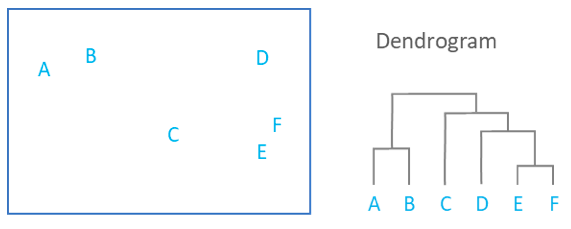
\includegraphics[width=\textwidth]{dendrogram}

It can be interpreted as each leaf being an observation and each fusion of two branches correspond to two observations/branches that are similar to each other. The height that these fusion occur corresponds to how similar they are. Using the image, We can say $E$ and $F$ are most similar. $D$ is similar to $E$ and $F$, but not as similar as $A$ is to $B$, since it is higher up on the dendrogram. To derive clusters from a dendrogram we make a horizontal cut anywhere on the y-axis and the first set of fusions directly below the cut (so not fusions that are below another fusion) are our clusters. If our cut crosses two lines then that corresponds to $K=2$ - we will have two clusters.

Hierarchical clustering assumes a hierarchical structure to the data - clusters obtained by cutting the dendrogram at a specific height are necessarily nested in clusters obtained by cutting the dendrogram at a greater height. E.g., a dataset of patients at a hospital who either do or do not have cancer and have type 1 or type 2 - with $K=2$ we naturally split on has cancer and does not and on $K=3$ we naturally split has cancer in to type 1 and type 2 - there is a hierarchy. Conversely, if we had a dataset of males and females from three different countries, splitting with $K=2$ might yield male and female, but $K=3$ would not split either male or female in to two new groups since nationality is not dependent on gender - there is no hierarchy in the data. When there is no hierarchy, hierarchical clustering can perform worse than k-means.

To build the dendrogram you first select a dissimilarity measure, e.g. Euclidean distance or correlation. The algorithm then treats each observation as its own cluster and finds the cluster with the least dissimilarity (most similarity) and creates (fuses) a new cluster. The algorithm then iteratively repeats this process, treating the previous fusion as a new cluster and removing the two clusters that were fused in to it from the pool. It continues until there is only 1 cluster ($K=1$) left. The dendrogram can be built from these fusions and uses how dissimilar the two clusters were when the fusion occurred to determine height.

The only problem here is determining the similarity between any object (single observation or a cluster) and a cluster. A cluster is made up of multiple observations so how do we determine similarity to a group. To do this there are 4 separate \textbf{linkage} schemes:

\begin{itemize}
    \item \textbf{Complete}: Complete linkage is the maximal inter-cluster dissimilarity - compute all pairwise dissimilarities between all observations in both clusters and select the maximum.
    \item \textbf{Single}: Single linkage is the minimal inter-cluster dissimilarity - compute all pairwise dissimilarities between all observations and select the minimum. This can result in extended, trailing clusters in which single observations are fused one at a time (more emphasis put on observation-observation fusions than observation-cluster).
    \item \textbf{Average}: Average linkage is the mean inter-cluster dissimilarity - compute all pairwise dissimilarities between all observations and average them.
    \item \textbf{Centroid}: Centroid linkage is the dissimilarity between the centroid of each cluster. This can lead to undesirable \textbf{inversions} (where two clusters are fused at a height below either of the individual clusters).
\end{itemize}

In general, Average and complete are preferred over single linkage as they give more balanced dendrograms. Centroid is avoided due to the inversion issue but finds use in genomics.
